% q0010.tex — Beyond the IRR-ational Choice (NPV / IRR profiles)
\question{
  id        = {0010},
  title     = {Beyond the IRR-ational Choice},
  source    = {OBECON},
  year      = {2026},
  round     = {Seletiva IEO -- Phase A},
  language  = {English},
  topic     = {Finance},
  subtopic  = {Capital Budgeting / NPV--IRR},
  type      = {objective},
  statement = {%
    An analyst is evaluating two mutually exclusive investment projects,
    Project~A and Project~B. To compare them, the analyst has plotted their
    Net Present Value (NPV) profiles against a range of discount rates.

    \begin{center}
      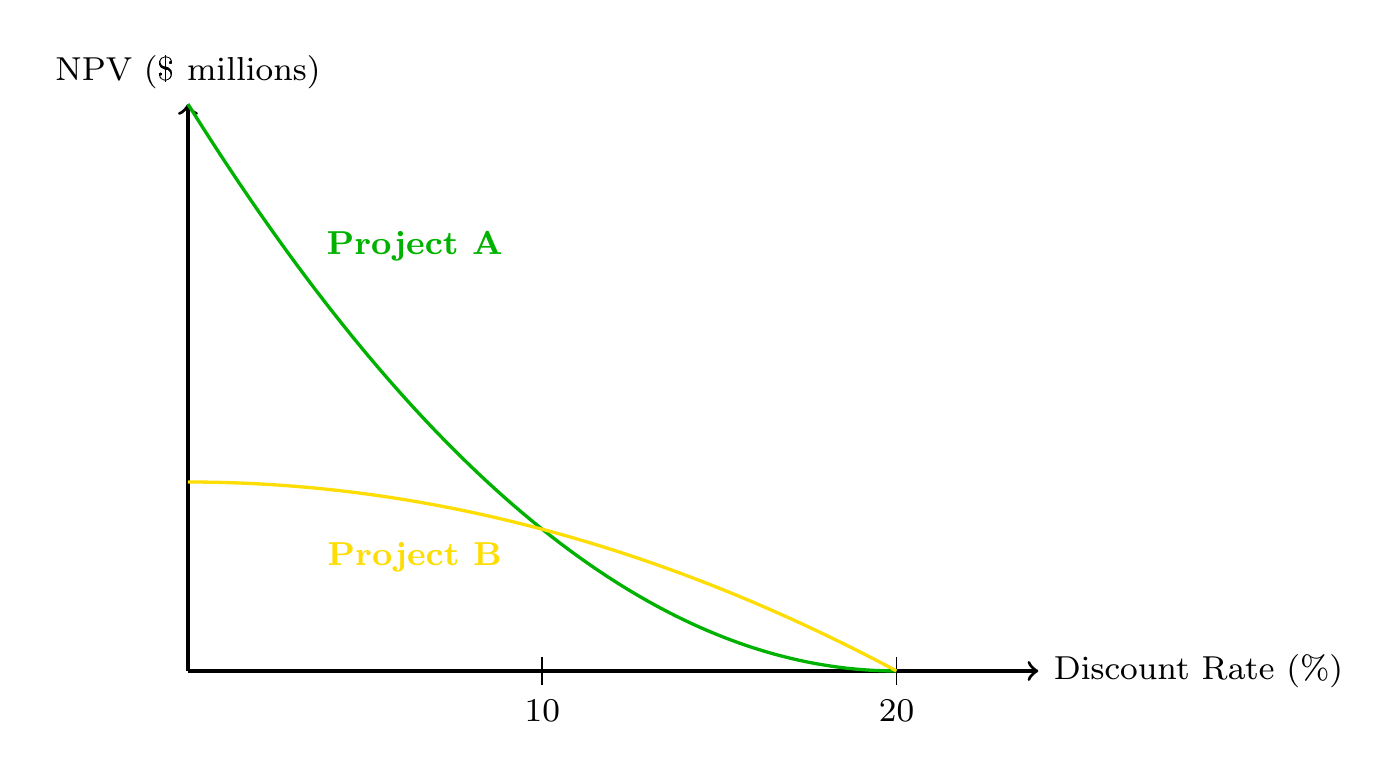
\includegraphics[width=0.72\textwidth]{../images/q0010_fig1.png}
    \end{center}

    Based on the NPV profiles above, which of the following statements is
    correct?
  },
  choices   = {%
    \item Project~A should be chosen, regardless of the cost of capital.
    \item Project~B should be chosen, regardless of the cost of capital.
    \item Both projects have an Internal Rate of Return (IRR) of 10\%.
    \item Both projects have an Internal Rate of Return (IRR) of 20\%.
    \item The choice depends on the cost of capital; Project~A is better if
          the rate is above a 10\% rate.
  },
  answer    = {D},
  solution  = {%
    Reading the NPV profile graph:
    \begin{itemize}
      \item Both curves cross the horizontal axis (NPV~$= 0$) at
            $r = 20\%$~$\Rightarrow$ \textbf{both projects have IRR~$= 20\%$}.
      \item The two curves intersect at $r = 10\%$ (the \emph{crossover
            rate} or Fisher intersection).
      \item For $r < 10\%$: Project~A has higher NPV~$\Rightarrow$ choose A.
      \item For $10\% < r < 20\%$: Project~B has higher NPV~$\Rightarrow$
            choose B.
      \item For $r > 20\%$: both NPVs are negative.
    \end{itemize}

    Option (E) is wrong because A is better \emph{below} 10\%, not above.
    Options (A) and (B) are wrong because the best choice depends on $r$.
    Option (C) is wrong: the IRR is 20\%, not 10\%.

    Answer: \textbf{(D)}.
  },
}
